\newpage
\section{XOR异或问题}
\begin{table}[htbp]
  \centering
  \caption{XOR问题}
    \begin{tabular}{ccc}
    \toprule
    \multicolumn{2}{c}{\textbf{Input}} & \textbf{Output} \\
    \midrule
    0     & 0     & 0 \\

    \rowcolor[rgb]{0.973, 0.973, 0.973} 0     & 1     & 1 \\

    1     & 0     & 1 \\

    \rowcolor[rgb]{0.973, 0.973, 0.973} 1     & 1     & 0 \\
    \bottomrule
    \end{tabular}%
  \label{XOR}%
\end{table}%

\subsection{二次函数代价函数}
%\[\begin{array}{l}
%E = \frac{1}{m}\sum\limits_x {{{\left\| {{a_3} - y} \right\|}^2}} \\
%\frac{{\partial E}}{{\partial {a_3}}} = \frac{2}{m}\sum\limits_x {({a_3} - y)} \\
%{\delta _3} = \frac{{\partial E}}{{\partial {z_3}}} = \frac{2}{m}\sum\limits_x {({a_3} - y)}  \odot \sigma '({z_3})\\
%{\delta _2} = {w_3}^T{\delta _3} \odot \sigma '({z_2})\\
%\frac{{\partial E}}{{\partial {b_2}}} = {\delta _2}\\
%\frac{{\partial E}}{{\partial {w_2}}} = {\delta _2}{a_1}^T
%\end{array}\]
首先我们选用二次函数作为代价函数
\begin{figure}[H]
\centering
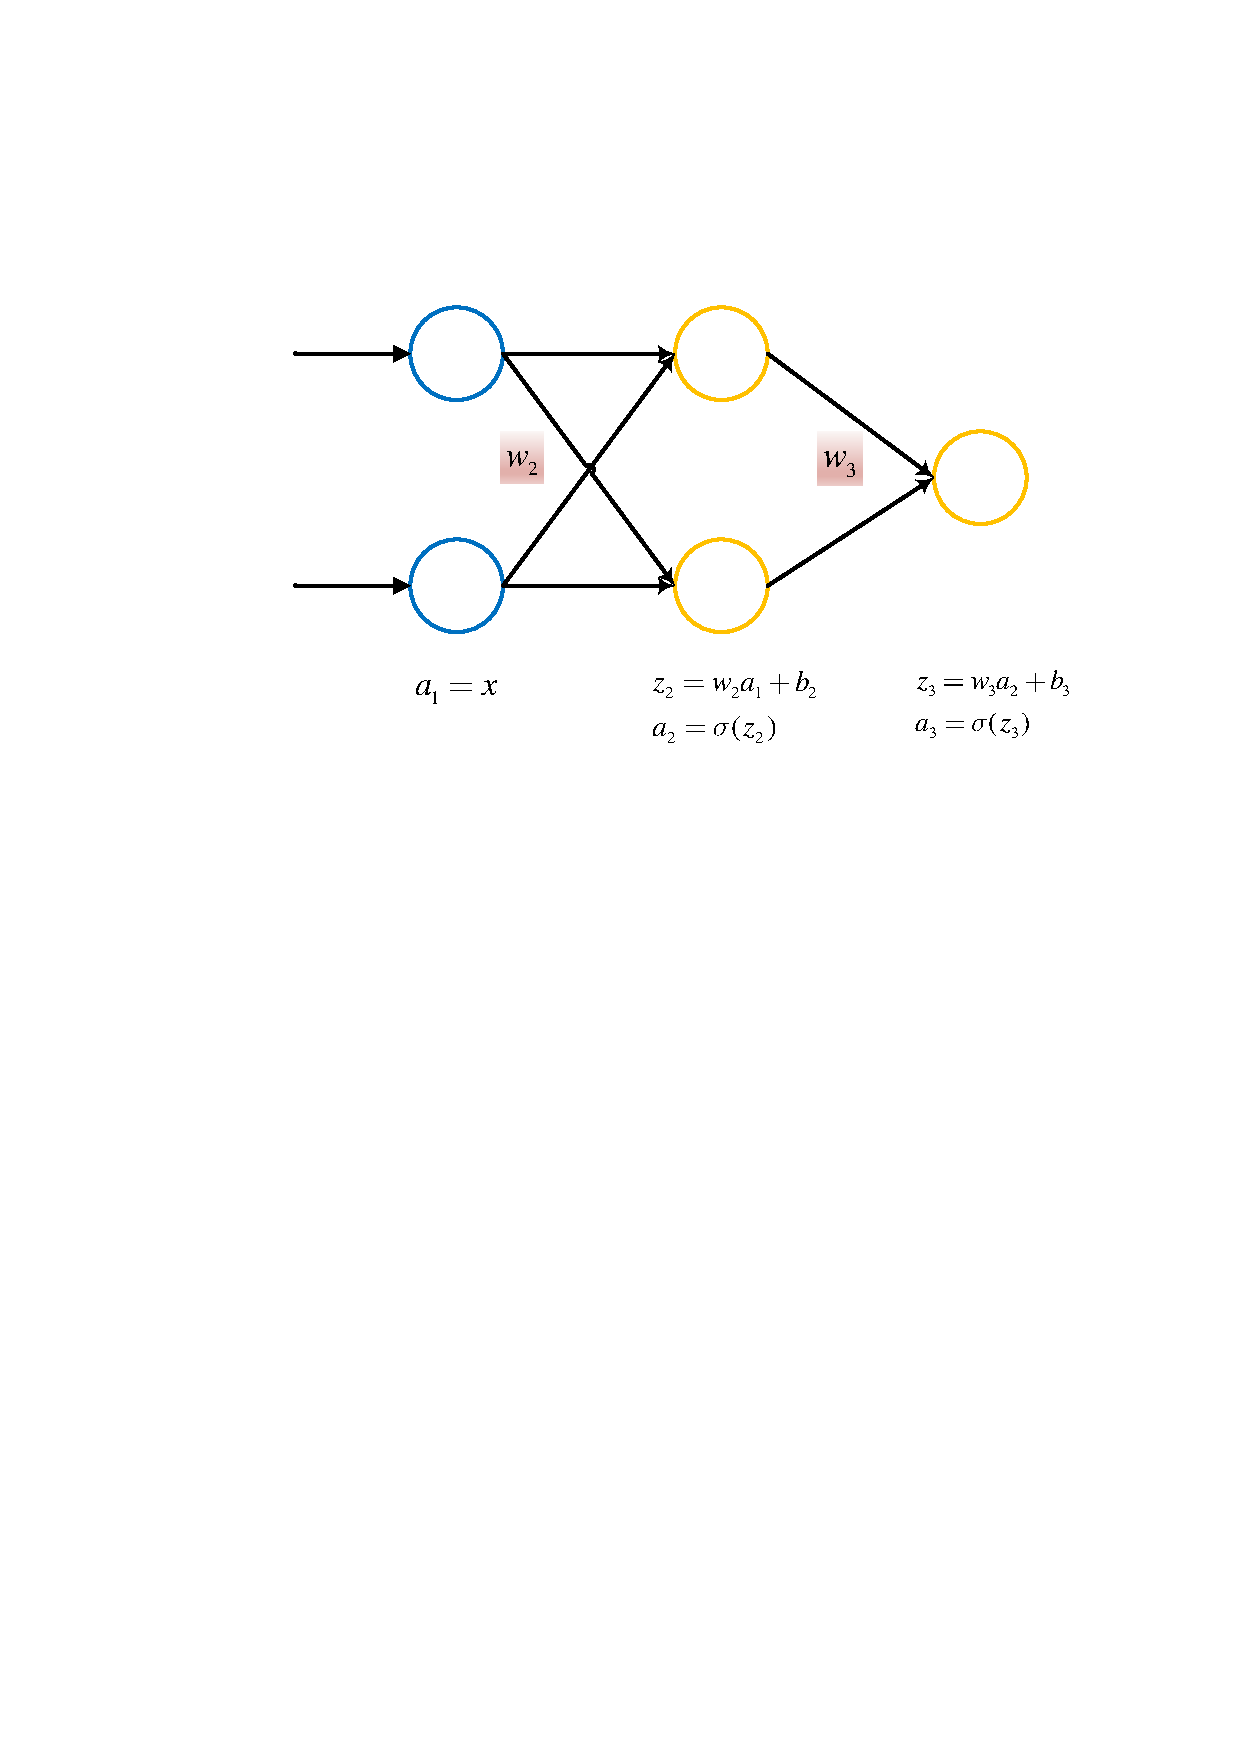
\includegraphics[width=8cm]{fig/Feedforward.pdf}
\caption{前向传播过程}
\end{figure}
\begin{lstlisting}
% Feedforward 前向传播计算成本函数
% w2大小 2 x 2
% w3大小 1 x 2
a1 = T'; 					% 输入层 a1大小 2 x 4
z2 = w2*a1+b2; 			% 第二层输入 z2大小 2 x 4
a2 = sigmoid(z2); 			% 第二层输出
z3 = w3*a2+b3;		% 第三层输入 z3大小 1 x 4
a3 = sigmoid(z3);			% 输出层 得到 1 x 4 的矩阵
cost = (a3-P').^2;
J(i) = sum(sum(cost, 2)) / m; 	% 求和得成本函数
\end{lstlisting}

\begin{figure}[H]
\centering
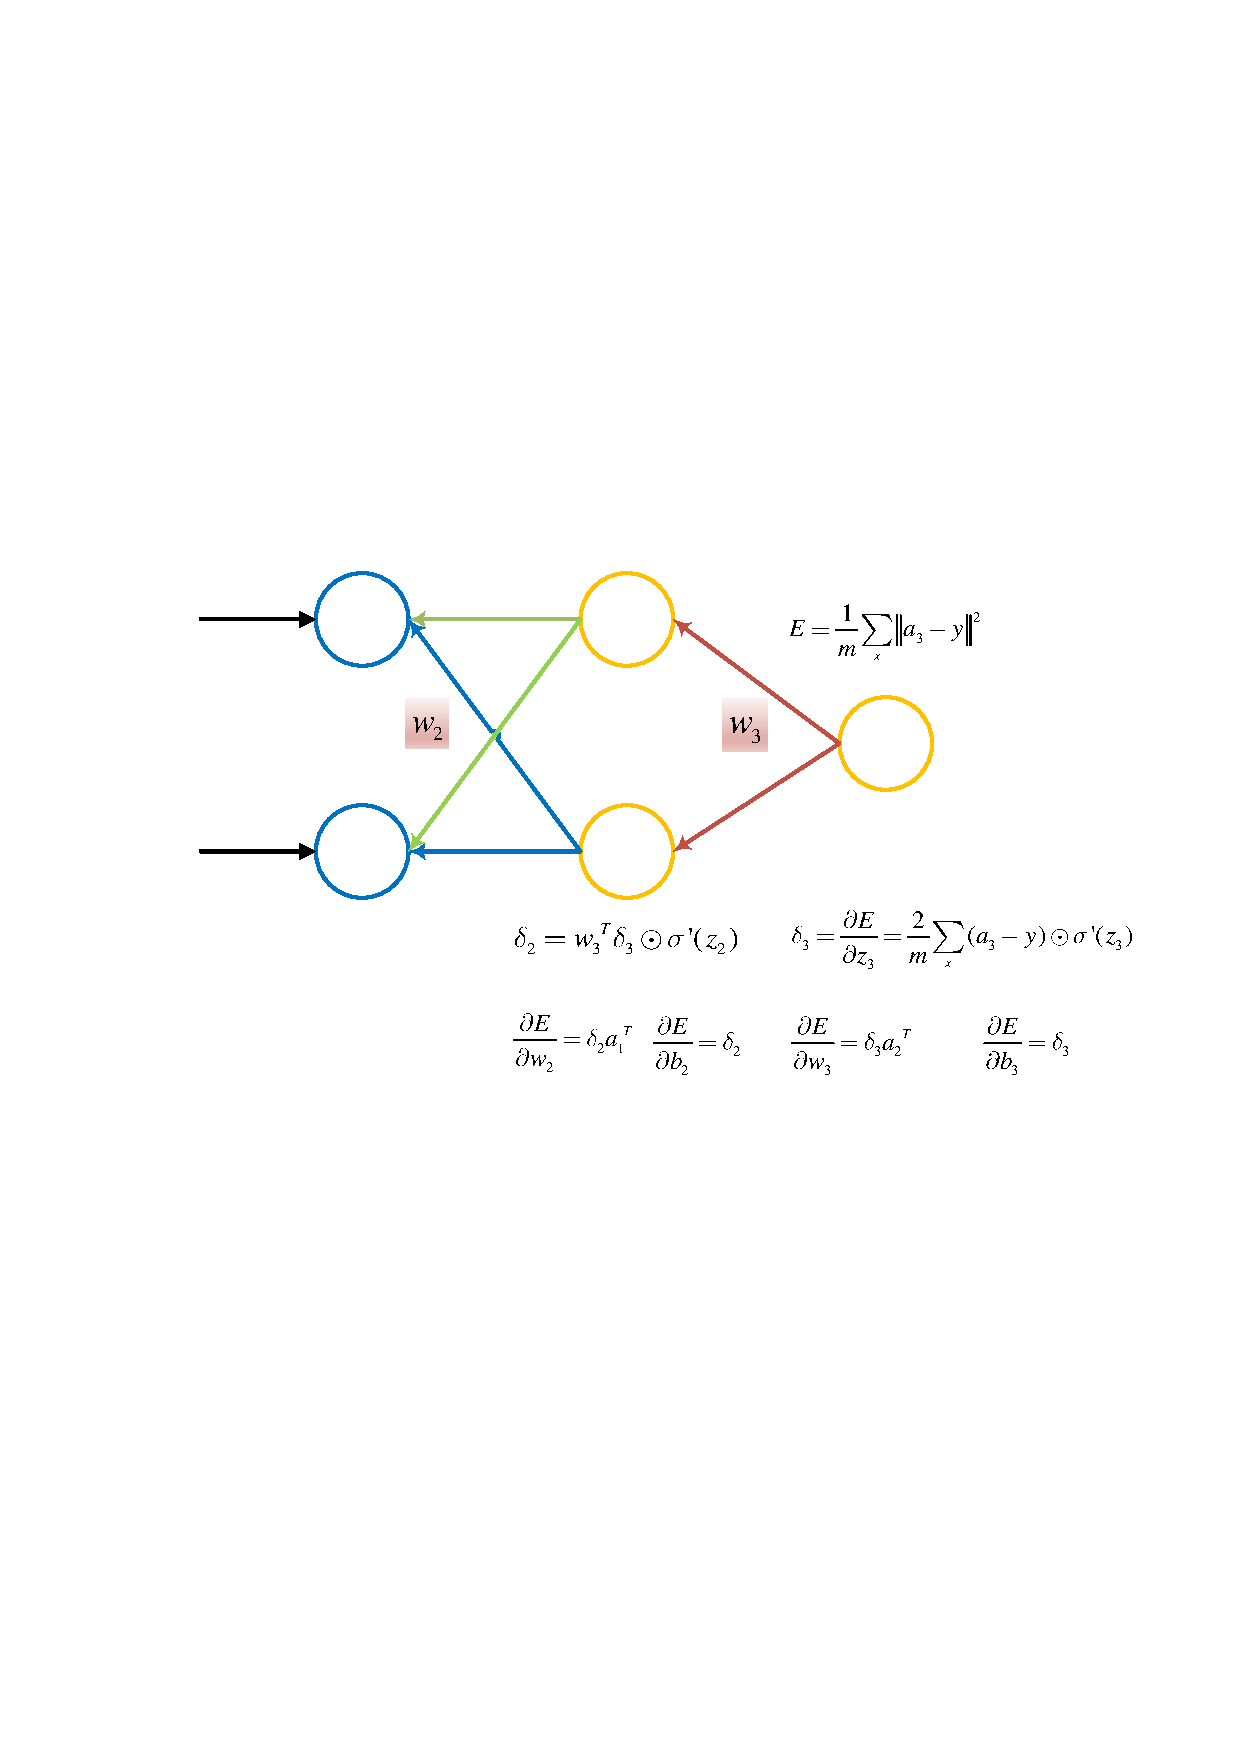
\includegraphics[width=13cm]{fig/Backpropagation.pdf}
\caption{反向传播过程}
\end{figure}

\begin{lstlisting}
% Backpropagation  反向传播计算梯度
Error3 =2/m*(a3-P').*d_sigmoid(z3); % 第三层的误差
Error2 = (w3)'*Error3.* d_sigmoid(z2);	% 第二层的误差

d_w3= Error3*a2'; % w2的梯度
d_b3= sum(Error3,2); % b3的梯度

d_w2= Error2*a1'; % w2的梯度
d_b2=sum(Error2,2); % b2的梯度
\end{lstlisting}


\begin{lstlisting}
%最后得到的各参数如下
w2 =
    5.6991    5.7146
    3.6140    3.6171

w3 =
    7.3065   -7.9139

b2 =
   -2.3530
   -5.5318

b3 =
   -3.2858

a3 =
    0.0640    0.9404    0.9404    0.0647

ans =
    0.0038
\end{lstlisting}

\begin{figure}[H]
\centering
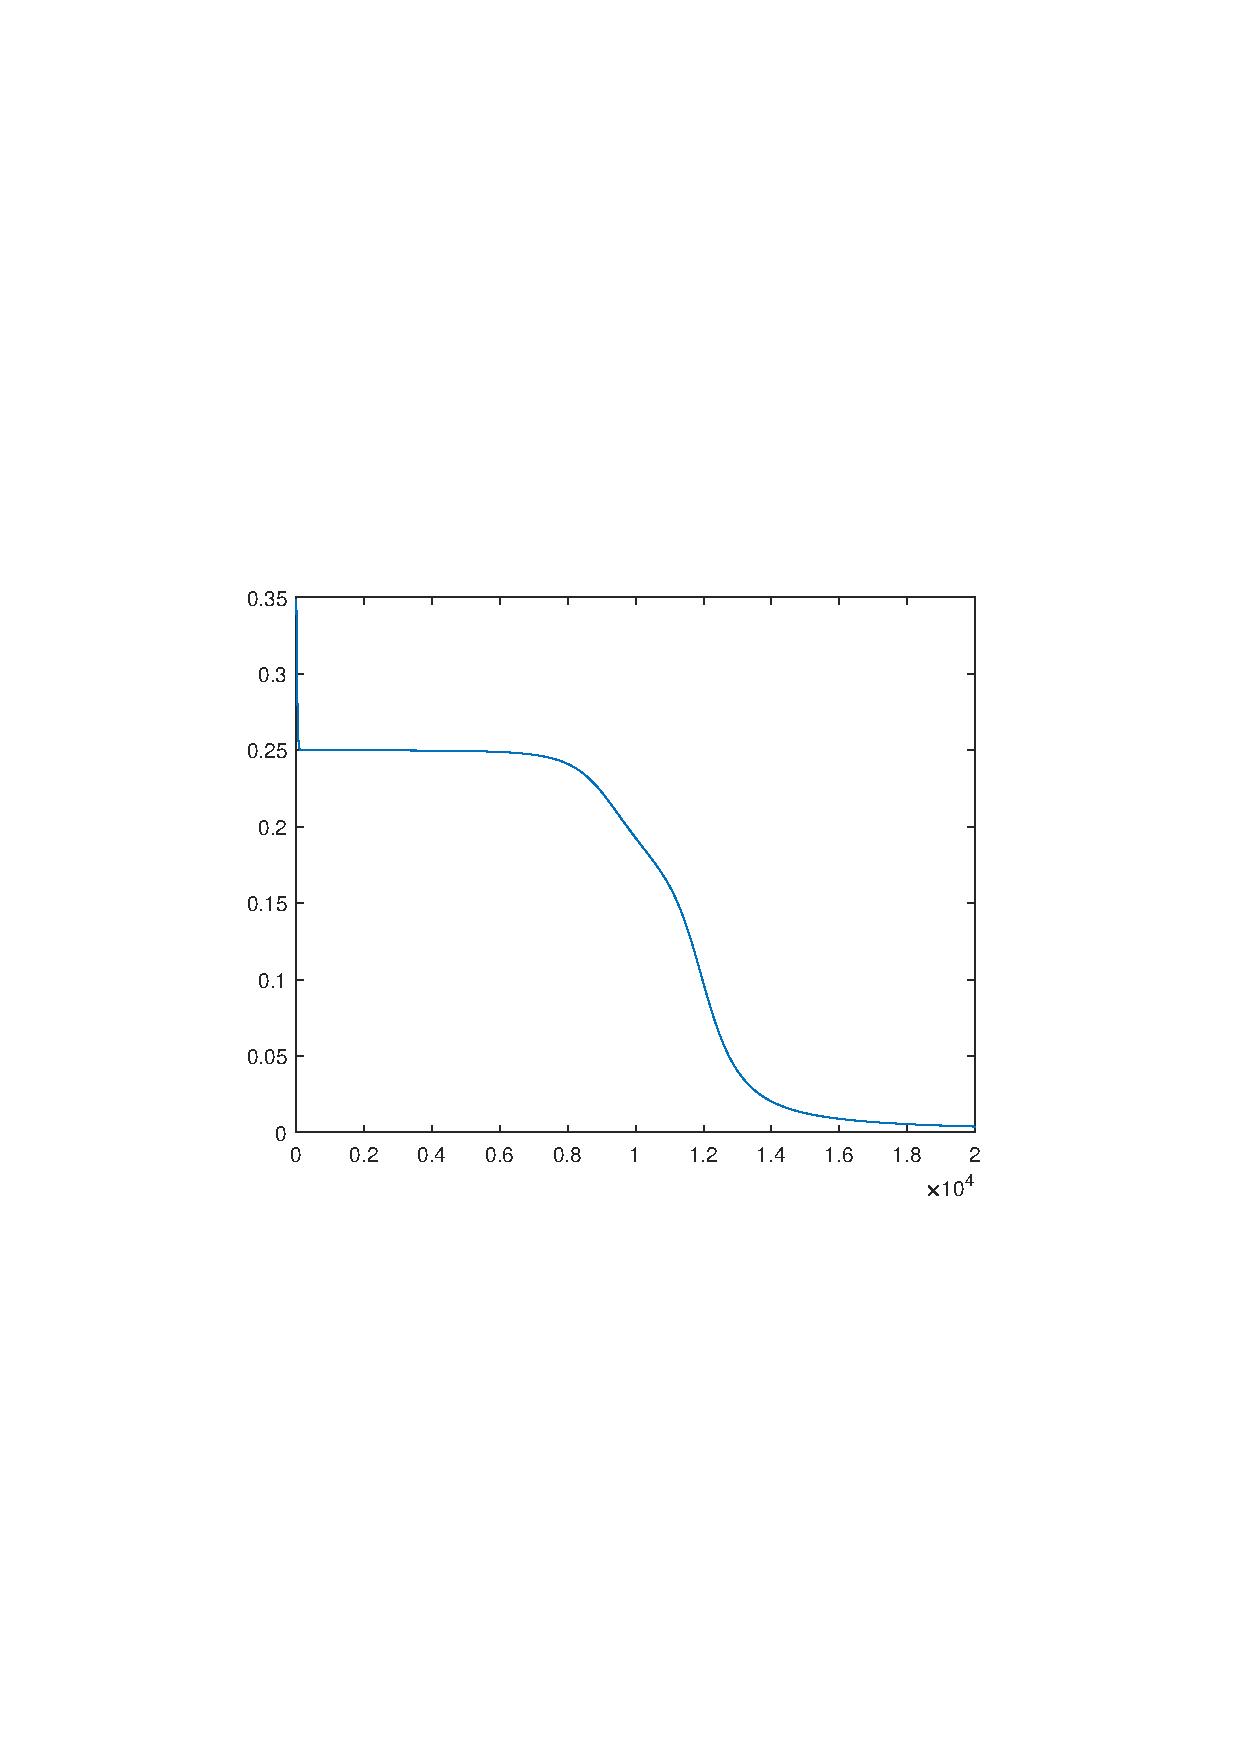
\includegraphics[width=10cm]{fig/xor1.pdf}
\caption{cost函数下降过程}
\end{figure}

观察图像我们可以发现:在刚开始迭代时,代价函数下降得非常快,但是在之后的前8000次迭代中,代价函数几乎没有下降,随后又突然急速下降,这是因为二次损失函数和Sigmoid激活函数组合时会发生\textbf{梯度消失}的现象.

下面我举一个简单的感知机例子来说明这种现象:
我们的输入为1,期望输出为0,将该感知机的权重和阈值初始化为0.6和0.9,那么第一次输出的结果为0.82,我们将学习速率定为$\eta=0.15$,迭代300次后停止,得到结果如下:
\begin{figure}[H]
\centering
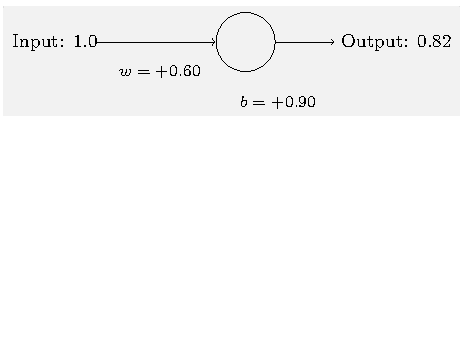
\includegraphics[width=8cm]{fig/1.pdf}
\caption{感知机}
\end{figure}

\begin{figure}[H]
\centering
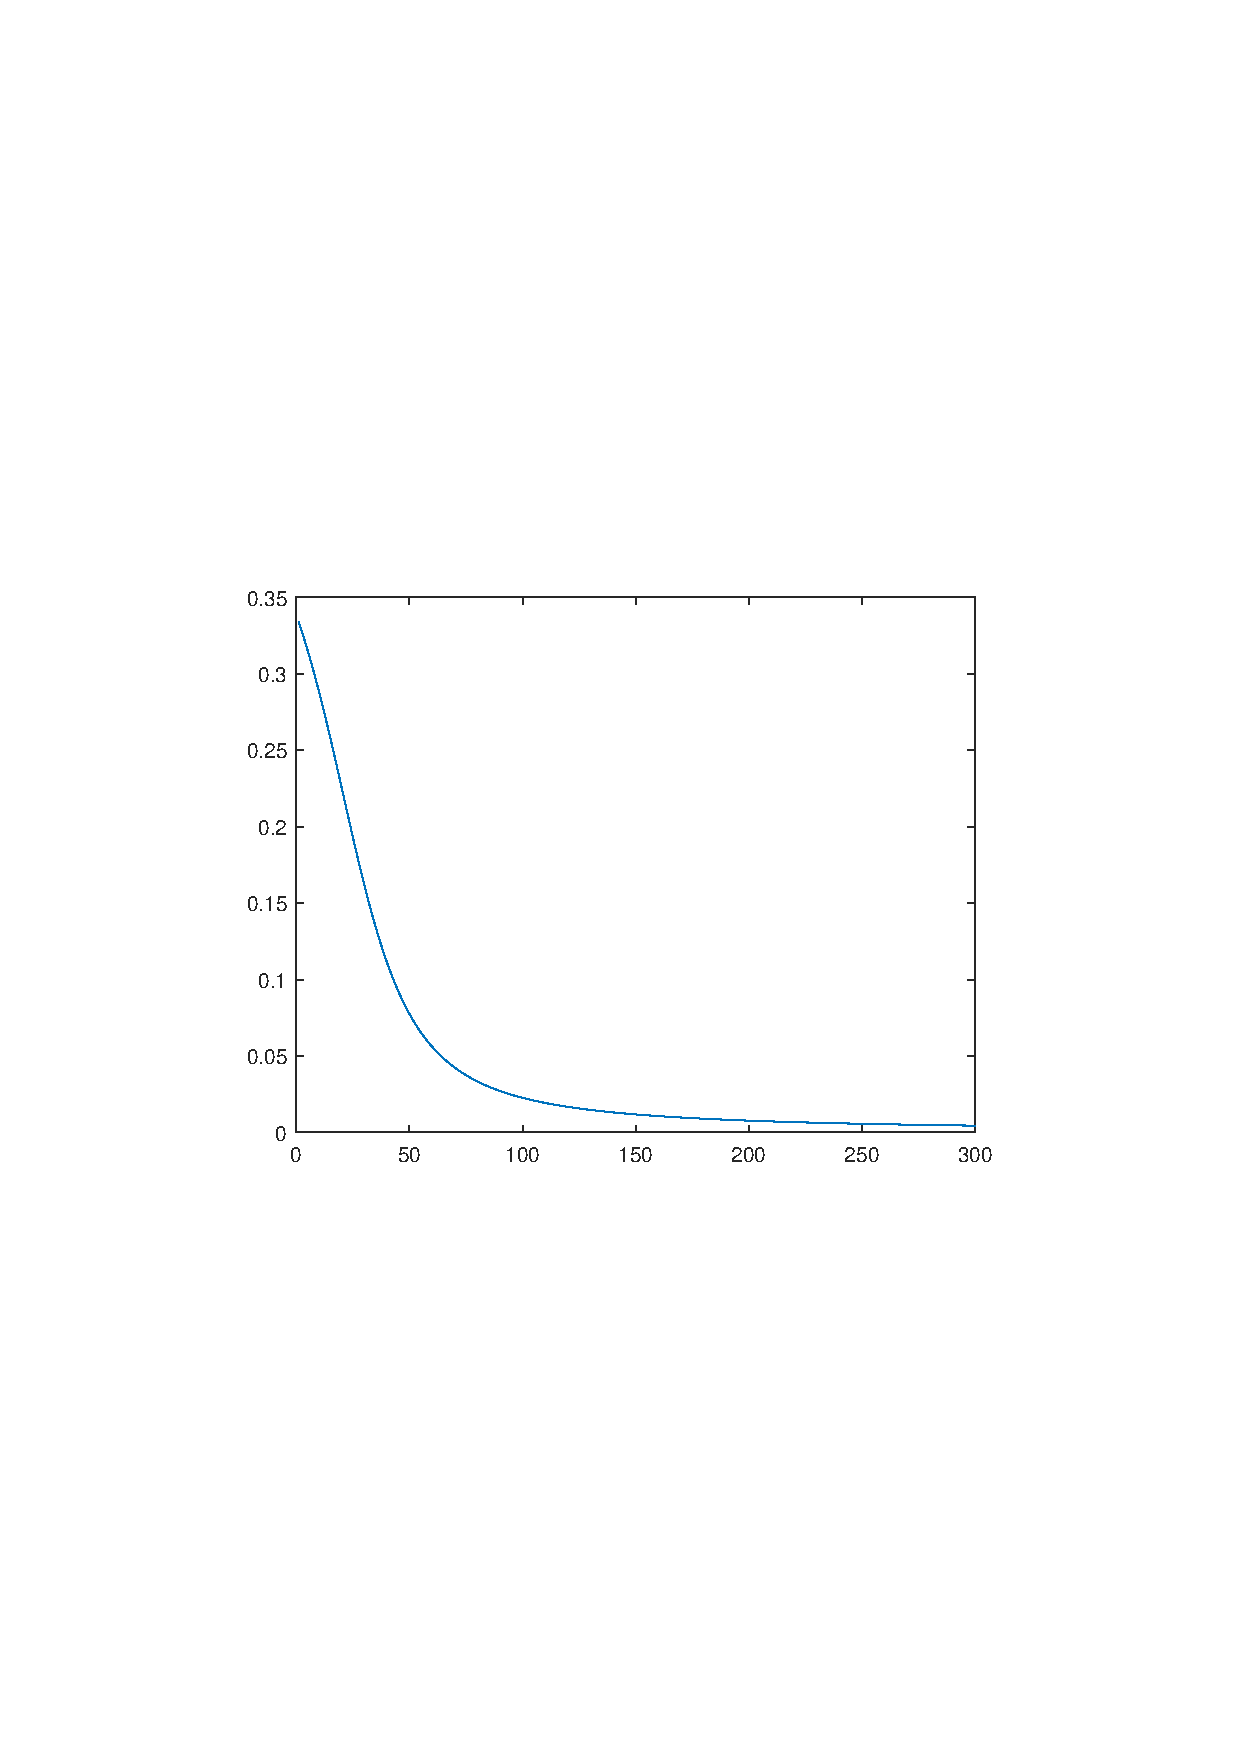
\includegraphics[width=7cm]{fig/test1.pdf}
\caption{初始化参数:$w=0.6,b=0.9$}
\end{figure}
这时我们看到感知机是像我们期望的那样快速收敛的,
但如果我们将感知机的权重和阈值初始化为2和2,
迭代结果却不一样了:

\begin{figure}[H]
\centering
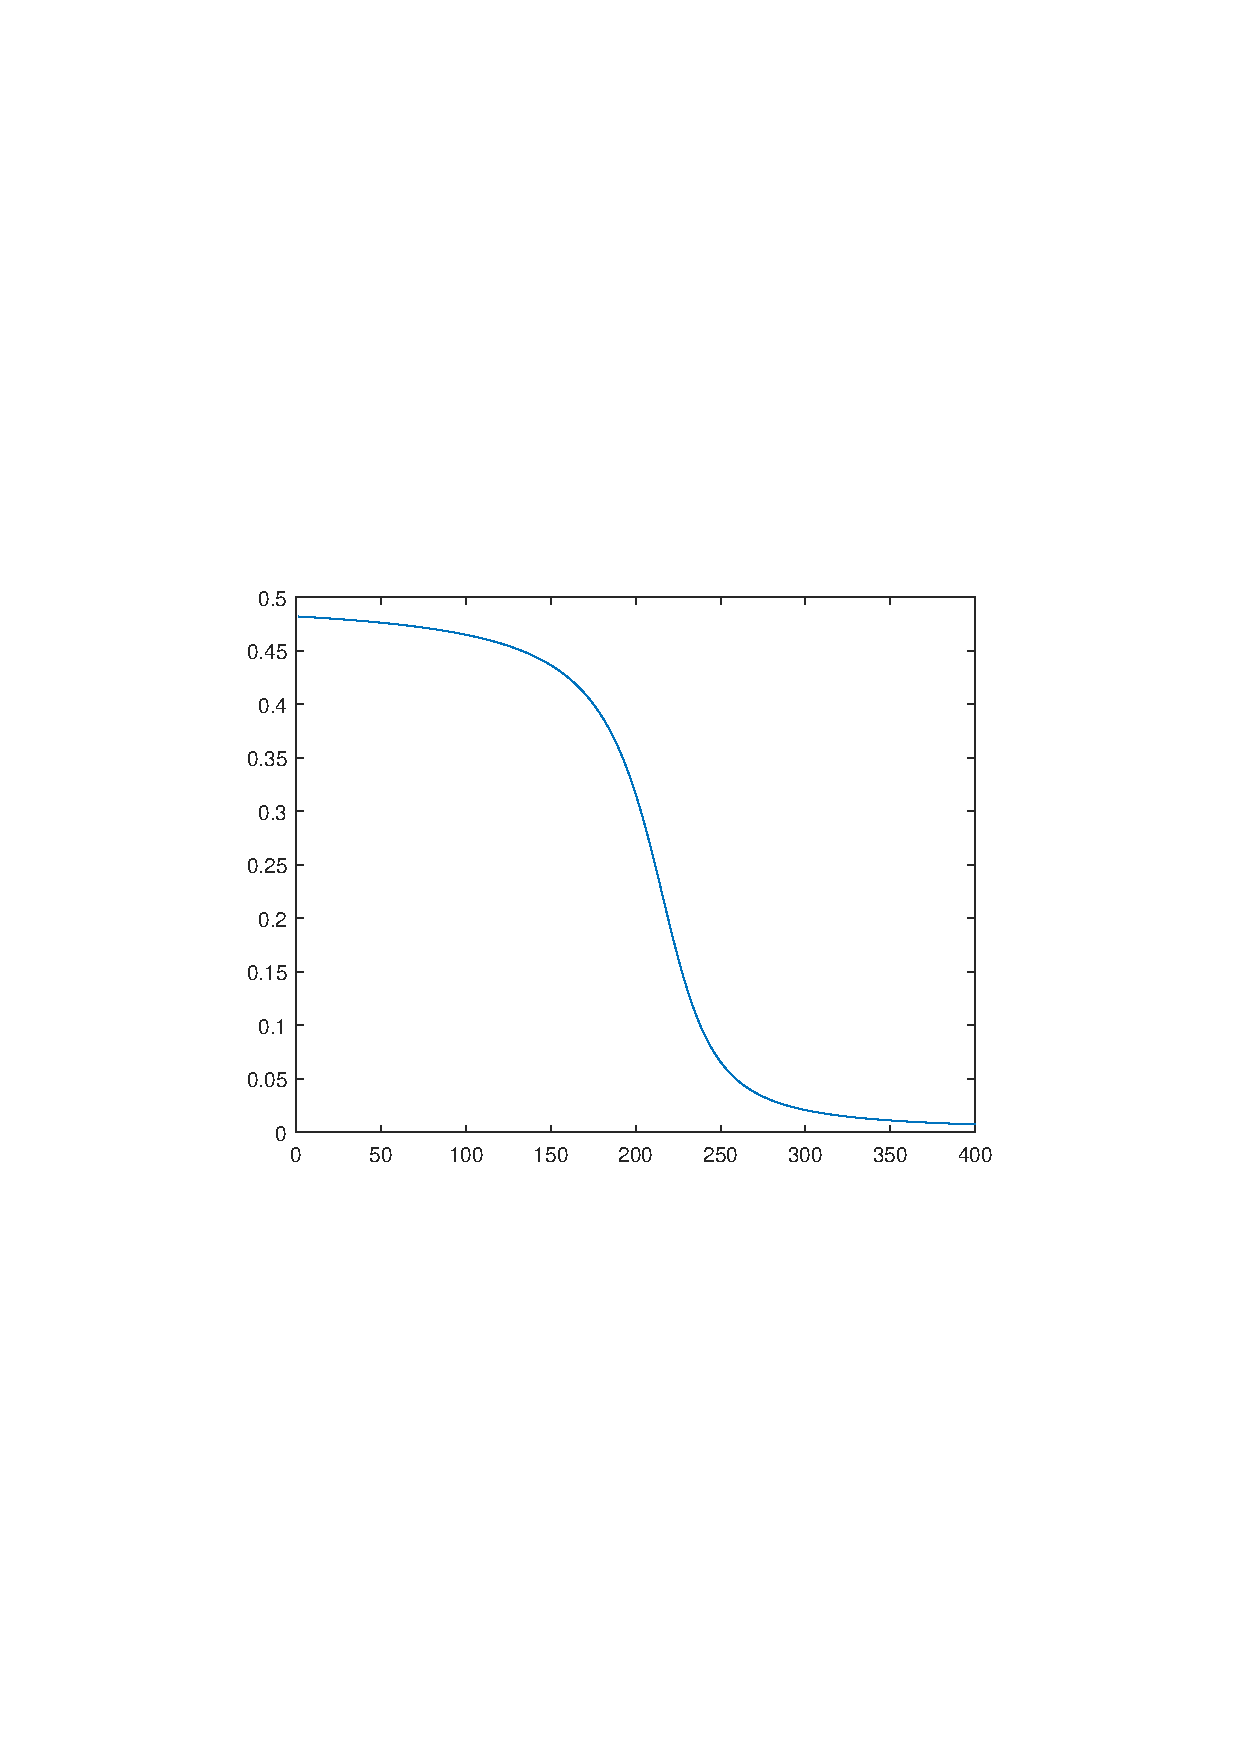
\includegraphics[width=7cm]{fig/test2.pdf}
\caption{初始化参数:$w=2,b=2$}
\end{figure}

图像呈现出来的结果也是先平缓下降,然后才加速,最后再减速。


\[E = \frac{1}{2}({a} - y)^2 \]
\begin{equation}
\frac{{\partial E}}{{\partial {w}}} = {a}\sigma'({z})x={a}\sigma'({z}) \label{dw1}
\end{equation}
\begin{equation}
\frac{{\partial E}}{{\partial {b}}} = a\sigma'({z}) \label{db1}
\end{equation}

\[\sigma'({z})=\sigma({z})(1-\sigma({z}))\]

从迭代公式中可以看出:当$\sigma({z})\rightarrow1\quad or\quad \sigma({z})\rightarrow0$时,$w,b$的梯度将会变得非常小,这会导致学习速率的缓慢,因此,我们可以将代价函数从二次函数替换为交叉熵函数,来改进神经网络。

\subsection{交叉熵代价函数}
定义代价函数为:
\[E = -y\ln a-(1-y)\ln (1-a) \]
那么可以求得:
\begin{equation}
\frac{{\partial E}}{{\partial {w}}} = (\sigma({z})-y)x \label{dw2}
\end{equation}
\begin{equation}
\frac{{\partial E}}{{\partial {b}}} = \sigma({z})-y \label{db2}
\end{equation}
对比等式(\ref{dw1})(\ref{dw2})可以发现:之前在二次代价函数里导致学习速率低的$\sigma'({z})$在等式(\ref{dw2})中刚好被消去了,并且这时学习速度也与误差$(\sigma({z})-y)$成正比了。

只要把原程序的$E,\partial E/\partial a_L$部分修改一下即可:
\begin{lstlisting}
cost = -P'.*log(a3)-(1-P').*log(1-a3);
J(i) = sum(sum(cost, 2)) / m; 	

Error3 =(a3-P')/m; 
\end{lstlisting}

交叉熵代价函数的下降过程如下:

\begin{figure}[H]
\centering
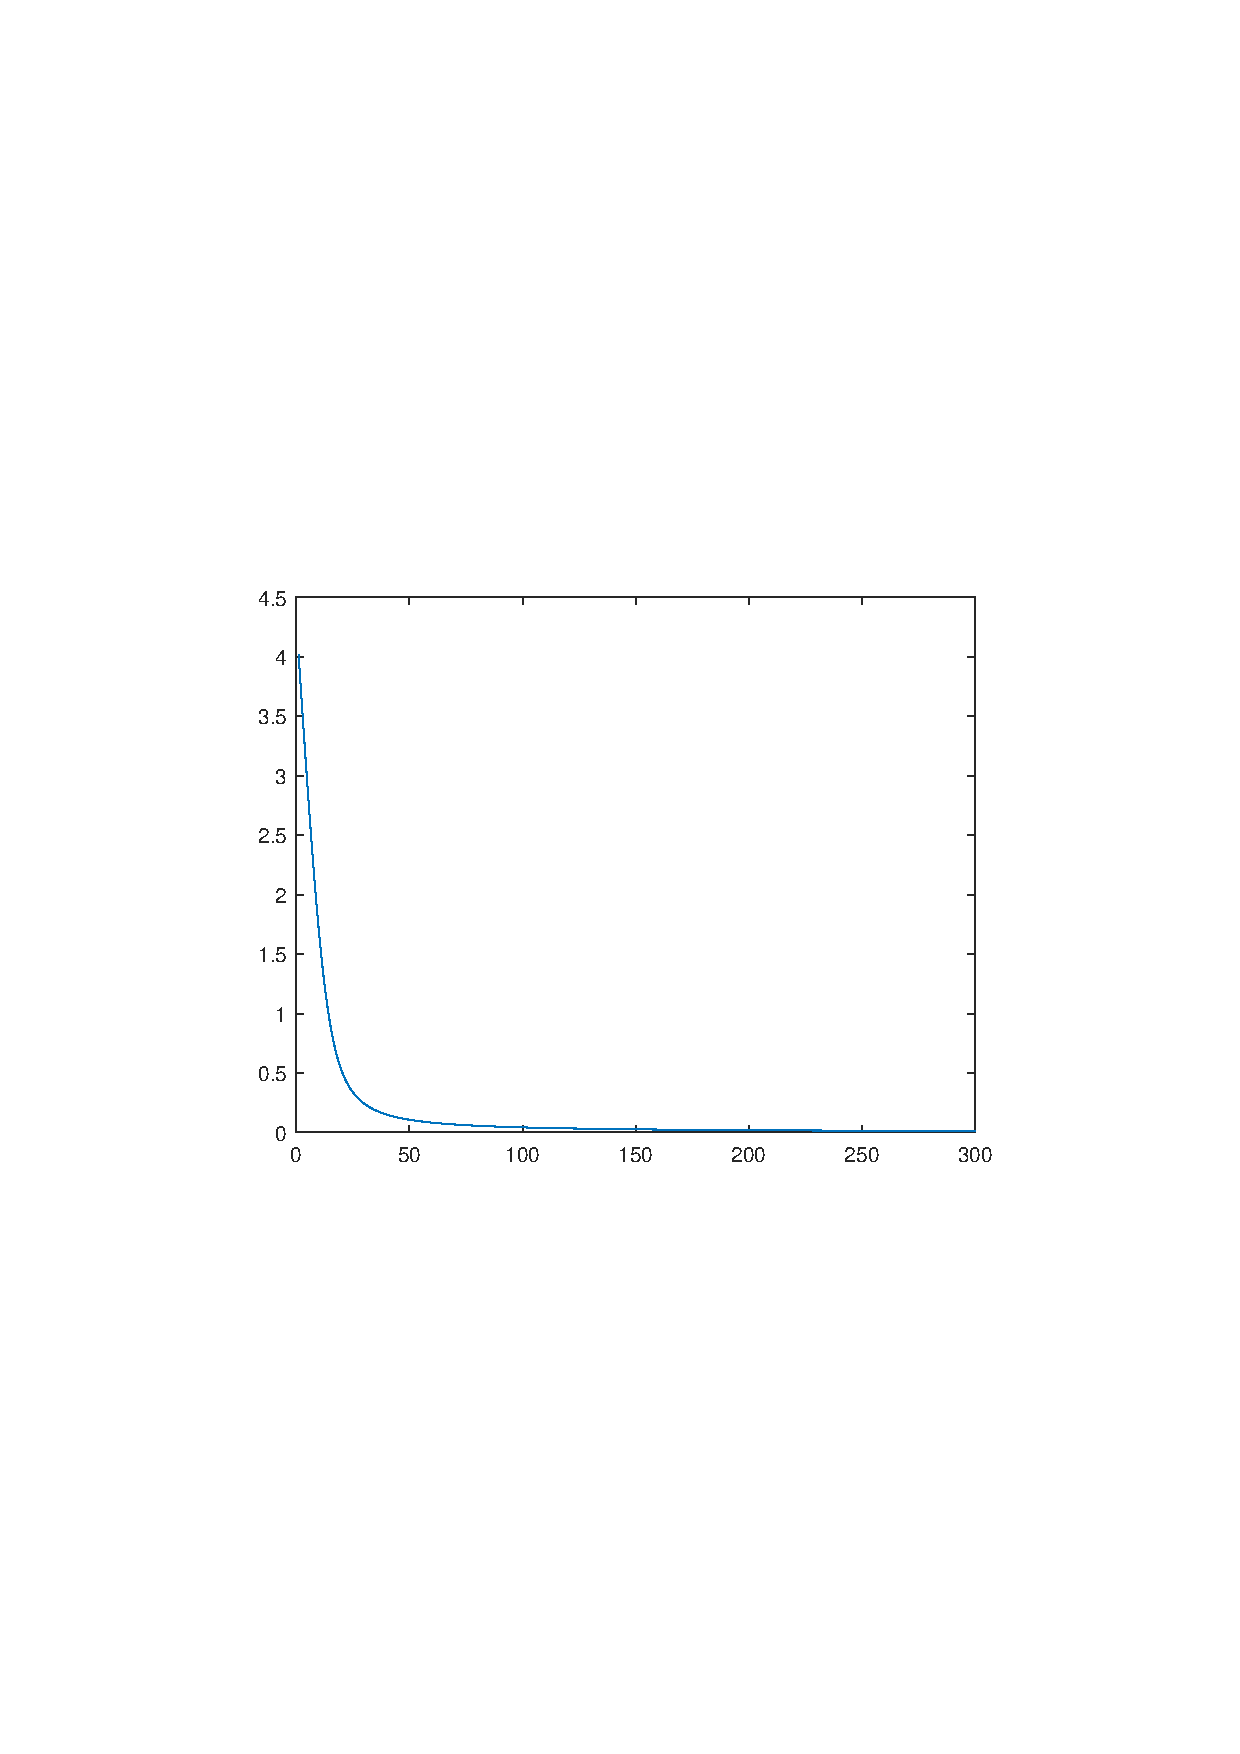
\includegraphics[width=8cm]{fig/test3.pdf}
\caption{交叉熵感知机程序}
\end{figure}

我们也能使用交叉熵代价函数来改造我们原来的xor程序,运行结果如下:
\begin{figure}[H]
\centering
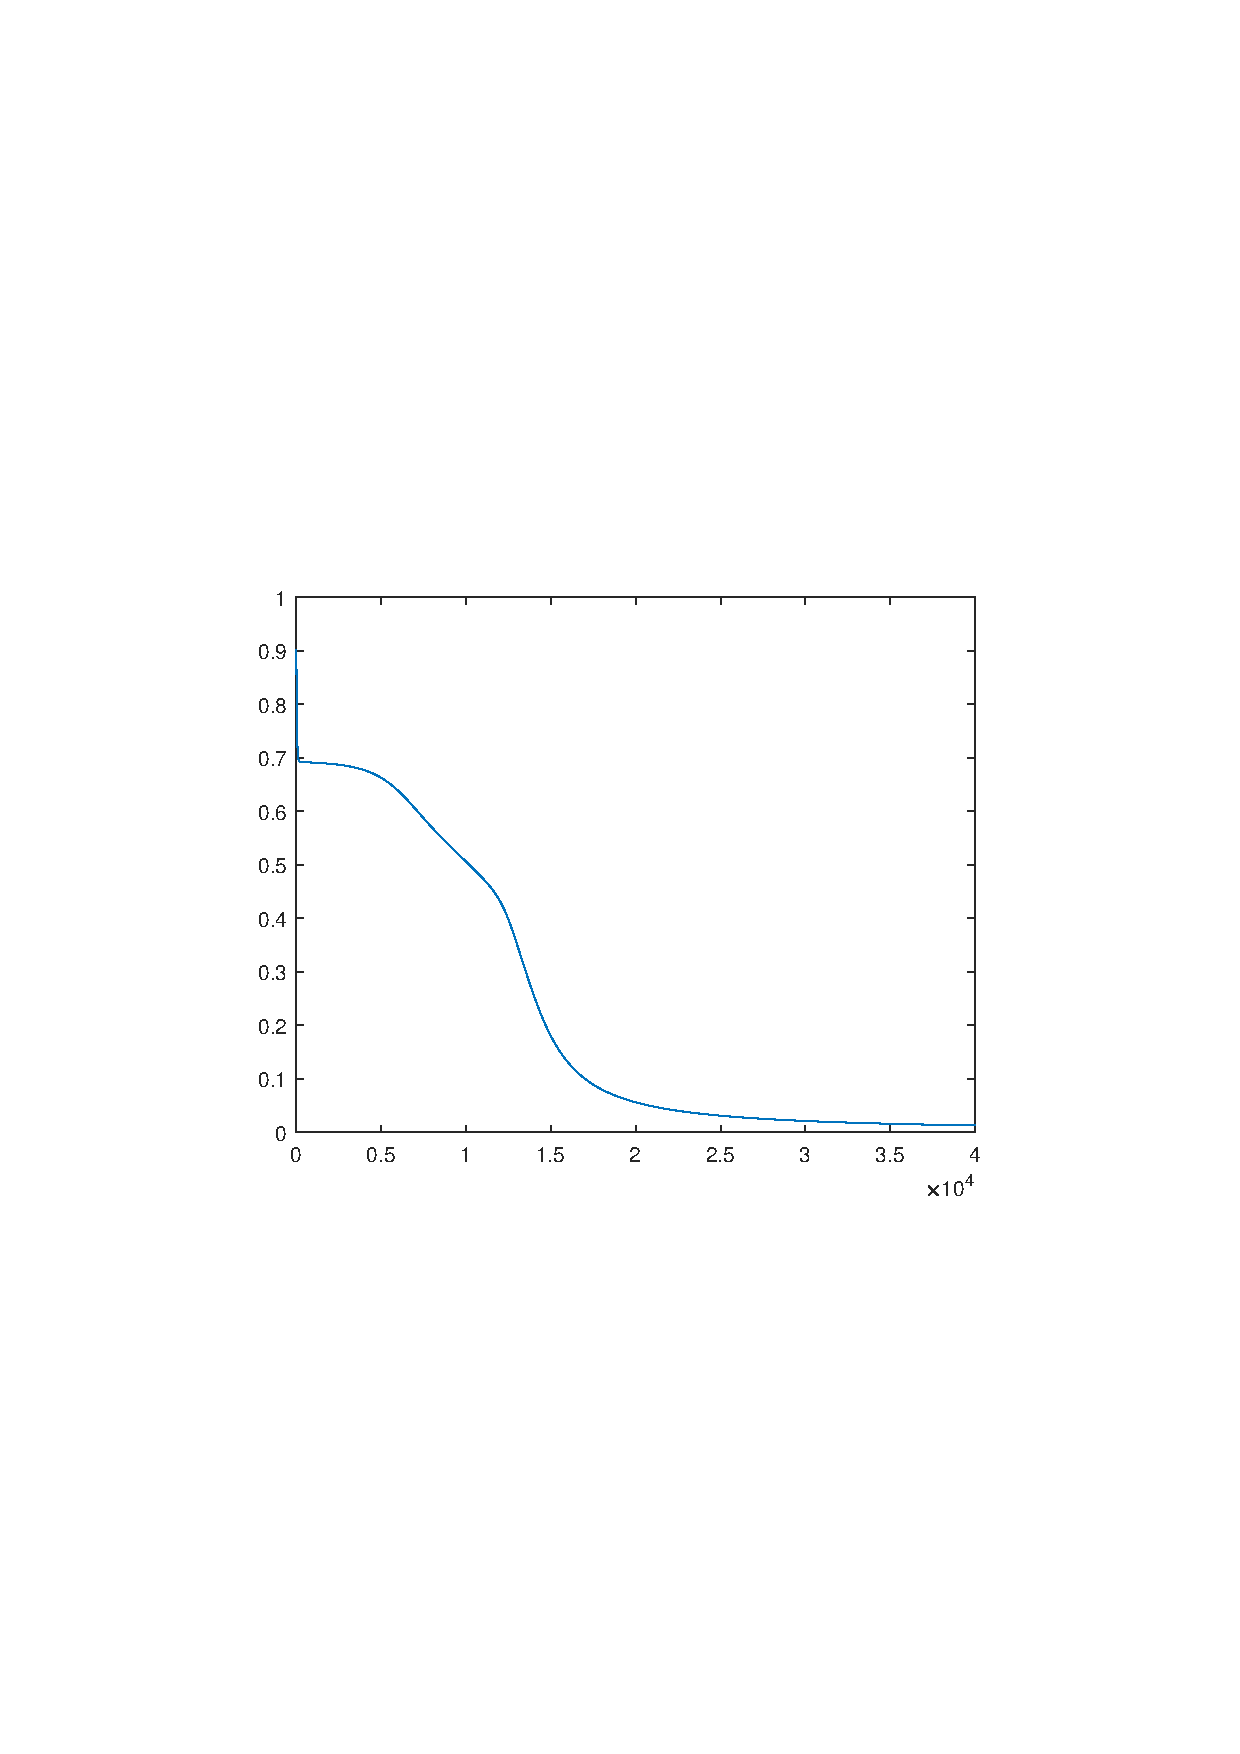
\includegraphics[width=8cm]{fig/xor2.pdf}
\caption{交叉熵xor程序}
\end{figure}
\newpage
\begin{lstlisting}
w2 =
    4.7028    4.6939
    6.8040    6.7488

w3 =
  -10.9213   10.1324

b2 =
   -7.1907
   -3.0075

b3 =
   -4.6355

a3 =
    0.0153    0.9883    0.9882    0.0129

ans =
    0.0130
\end{lstlisting}

\subsection{动量项momentum}
动量项是将梯度下降更新规则 $w\rightarrow w'=w-\eta\nabla E$ 改成
\begin{align} 
  v \rightarrow v' &= \mu v - \eta \nabla E \\
  w \rightarrow w' &= w+v' 
\end{align}


如果梯度在上一次迭代的方向和这一次的方向相同,那么,改变量就会叠加,
朝那个方向移动的速度就会增加,
而如果方向不同,那么则会抵消一部分,使得反方向运动的速度慢下来。
这个与物体运动中的惯性有些类似,因此称为动量项。

添加了动量项的xor程序运行结果如下:
\begin{lstlisting}
w2 =
    7.3616    7.3609
    5.4367    5.4366

w3 =
   12.3830  -13.2183

b2 =
   -3.3630
   -8.3198

b3 =
   -5.7669

a3 =
    0.0047    0.9966    0.9966    0.0035
    
ans =
    0.0037
\end{lstlisting}

\begin{figure}[H]
\centering
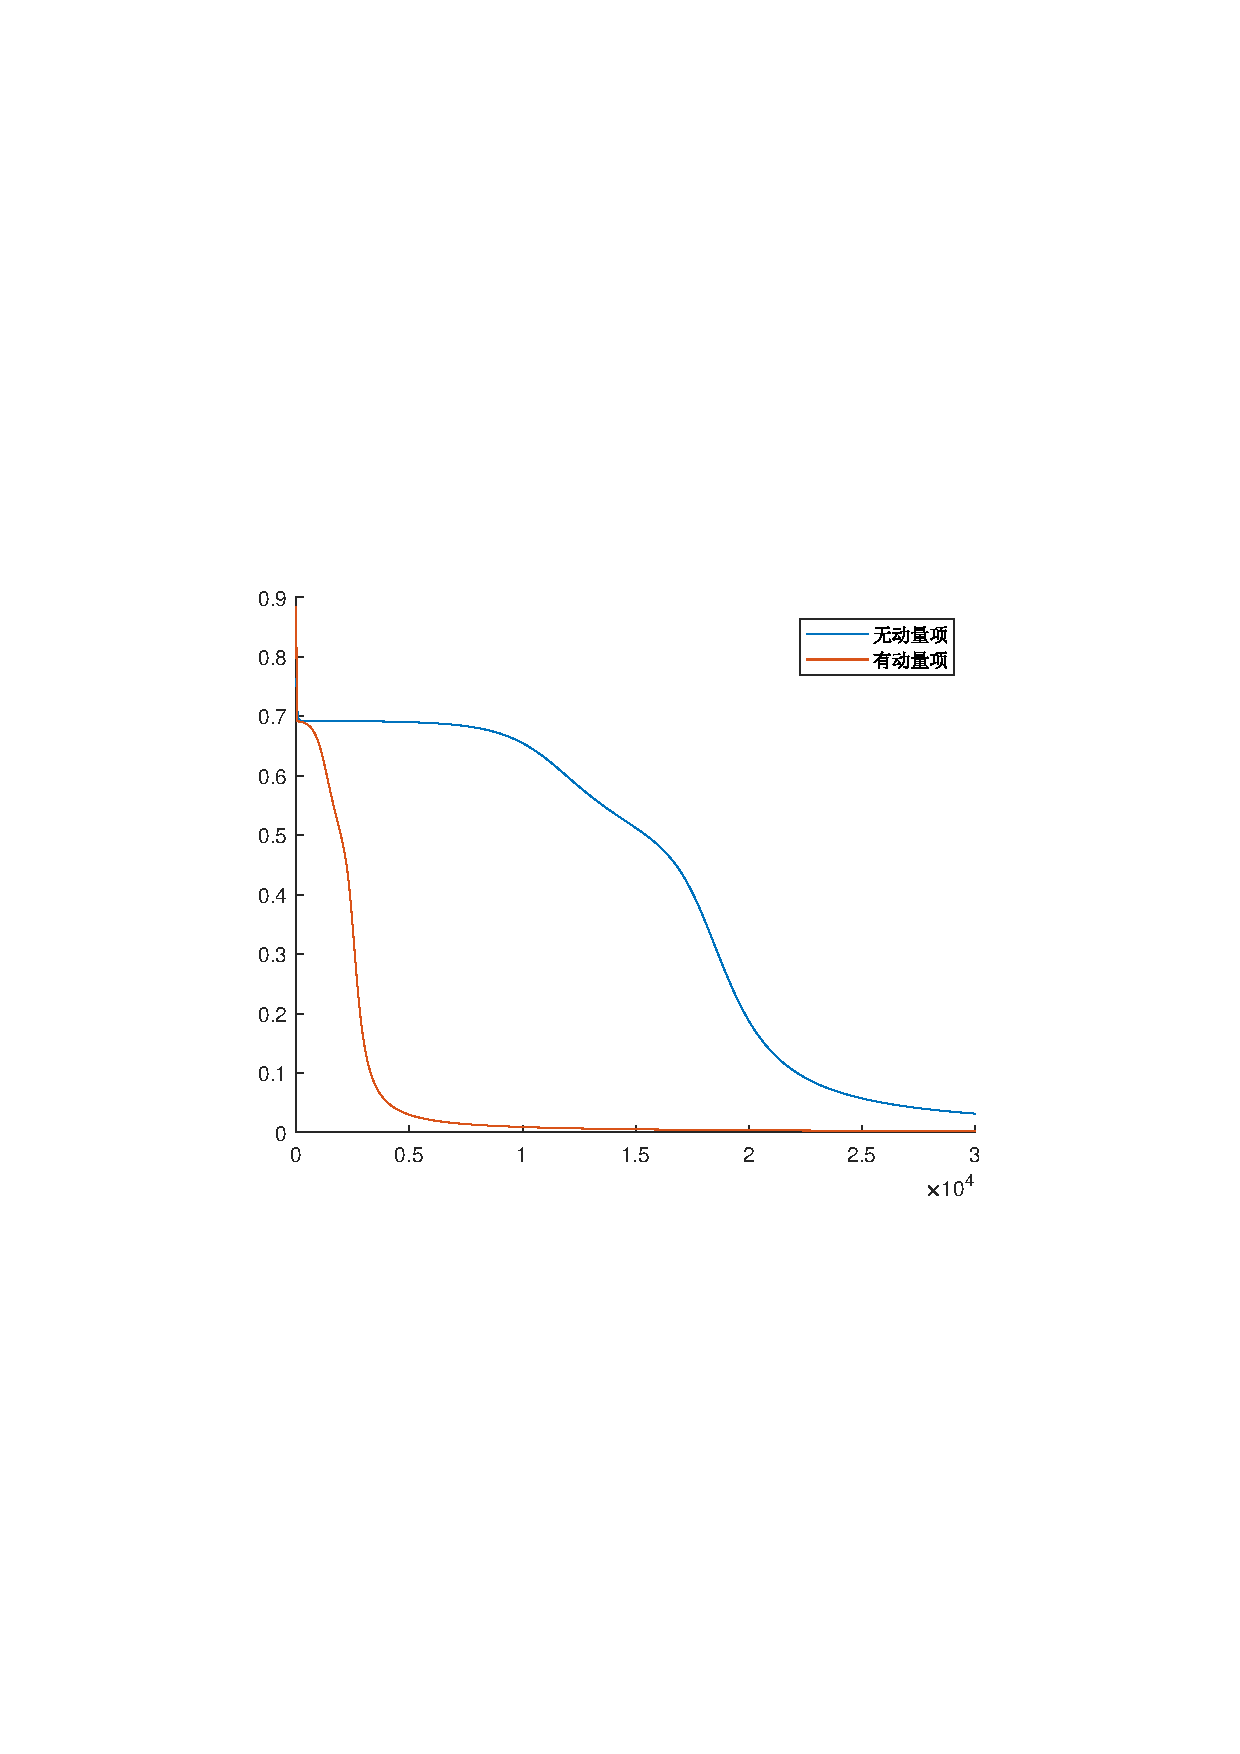
\includegraphics[width=10cm]{fig/compare.pdf}
\caption{对比}
\end{figure}

可以明显地看出,添加了动量项后,神经网络收敛的速度有了非常大的提升。